

\documentclass[letterpaper,twocolumn,amsmath,amssymb,prb]{revtex4-1}
\usepackage{graphicx}% Include figure files
\usepackage{dcolumn}% Align table columns on decimal point
\usepackage{bm}% bold math
\usepackage{color}

%%%%%%%%%%%%%%%%%%%%%%%%%%%%%%%%%%%%%%%%%%%%%%%%%%%%%%%%%%%%
%% Definitions
\def\re{\text{Re}}
\def\im{\text{Im}}
\def\ket#1{\vert #1 \rangle}
\def\cU{{\cal{U}}}
\def\cD{{\cal{D}}}
\def\re{\text{Re}}
\def\im{\text{Im}}
\newcommand{\red}[1]{{\bf \color{red} #1}}
\newcommand{\blue}[1]{{\bf \color{blue} #1}}
\newcommand{\green}[1]{{\bf \color{green} #1}}
\newcommand{\rr}{\textbf{r}}
\newcommand{\xx}{\textbf{r}}
\newcommand{\refnote}{\red{[ref]}}

\newcommand{\fixme}[1]{\red{[#1]}}

% needsworklater is used to annotate bits that need work, but that we
% can postpone for a while.
\newcommand{\needsworklater}[1]{\emph{[#1]}}
% needsworknow is intended to prioritize stuff that needs fixing.
\newcommand{\needsworknow}[1]{\textcolor{red}{[\emph{#1}]}}

%%%%%%%%%%%%%%%%%%%%%%%%%%%%%%%%%%%%%%%%%%%%%%%%%%%%%%%%%%%%

\begin{document}
\title{A Classical Density-Functional Theory for Describing Water Interfaces}

\author{Jessica Hughes}
\affiliation{Department of Physics, Oregon State University, Corvallis, OR
97331}

\author{David Roundy}
\affiliation{Department of Physics, Oregon State University, Corvallis, OR
97331}

%%%%%%%%%%%%%%%%%%%%%%%%%%%%%%%%%%%%%%%%%%%%%%%%%%%%%%%%%%%%
\begin{abstract}
{We develop a classical density functional theory for water by combining the
fundamental-measure theory functional--which describes hard sphere fluids--with
attractive interactions based on the Statistical Associating Fluid Theory
(SAFT). Using this approximation, we are able to describe the vapor pressure, 
various densities, surface tension, enthalpy and
entropy of water, as well as the number of hydrogen bonds formed near
liquid-vapor and liquid-solid interfaces. These interfaces include water
confined to a hard-walled slit, a single hydrophobic rod immersed in water, and
two hydrophobic rods 
at various separations. We found \needsworknow{conclusion-like stuff about two
rods, vapor-liquid transition between rods, constant force of twice surface
tension, more?}.
This functional provides a foundation for future work predicting the
interactions of chemicals in aqueous solution on an
atomic level.}

%\tableofcontents
\end{abstract}

\maketitle

%%%%%%%%%%%%%%%%%%%%%%%%%%%%%%%%%%%%%%%%%%%%%%%%%%%%%%%%%%%%
\section{Introduction}

\subsection{Water---the universal solvent}

The simple yet complex water molecule is one of the most important 
substances for life and industry. The structure and geometry of the 
water molecule leads to a strong polarity and complex intermolecular
forces. The hydrogen bonds formed by water are very strong, creating
tetragonal clusters that lead to many of water's unusual properties,
such as the high melting, boiling, and critical temperatures as well as the
density maximum above the melting point.
The large dielectric constant is partially responsible for
water acting as a universal solvent, along with the ease of availability and
use.
There are many models used to describe water since so many different
processes occur in aqueous solution. It is challenging to describe all the 
relevant properties of water at once, especially if a low computational cost is
also desired.

Some models are primarily designed for use with homogeneous systems. Although
these 
models are useful in predicting some bulk properties, the interesting
chemistry that occurs in water cannot be described with a homogeneous-only
model. To
describe solvation and other processes in aqueous solution, a more robust theory
that 
can handle varying densities is needed.

\subsection{Classical density-functional theory}

Classical density-functional theory (DFT) provides an efficient way to evaluate
the free energy using the probability distribution of the fluid. The free energy 
is a functional
of the density function and is independent of any external
potentials\cite{ebner1976density}. The most common use of DFT is calculating ground
state electron densities in quantum mechanical systems. The Hohenberg-Kohn
theorem\cite{hohenberg1964inhomogeneous} allows us to write the ground state
energy in terms of a universal functional of the electron density and a separate
term including the external potential. Mermin\cite{mermin1965thermal} gives a
theorem extending that of Hohenberg and Kohn to nonzero temperatures:
\begin{equation}
  A(T) = \underset{n(r)}{min}\left\{ F[n(r),T] + \int V_{ext}(r) n(r)
d^3r\right\}
\end{equation}
This is the basis for classical DFT, where the relevant density is not the
electron density,
but the density of molecules. This can be used with a variety of 
external potentials, from the simple interaction with a 
hydrophobic wall to the more complex, stronger interaction with hydrophilic
solutes.

\subsection{Statistical Associating Fluid Theory}

The high hydrogen bonding and strong polar interactions in water characterize it
as an associating fluid, and thus it requires a different treatment than simple
fluids which are mainly defined by van der Waals forces and weak electrostatic
interations. The Statistical Associating Fluid Theory (SAFT) was designed for
use with fluids such as water, to account for the important association forces
(like hydrogen bonds) as well as any effects due to clusters or chains forming
in the liquid\cite{muller2001molecular}. It is based on Wertheim's first-order
thermodynamic perturbation theory (TPT1)
\cite{wertheim1984fluidsI,wertheim1984fluidsII,wertheim1986fluidsIII,
wertheim1986fluidsIV} which provides a useful way to account for strong
associative interations between molecules.

%%%%%%%%%%%%%%%%%%%%%%%%%%%%%%%%%%%%%%%%%%%%%%%%%%%%%%%%%%%%
\section{Theory and Methods}
We introduce a new classical density functional for water that
predicts the vapor density, liquid density, and bulk surface tension, as well 
as allows for liquid-vapor coexistence.  The Helmholtz free energy functional is
based on SAFT, and is composed of the usual terms:
\begin{equation}
  F[n] = F_\textit{id}[n] + F_\textit{hs}[n]  +
F_\textit{disp}[n]+ F_\textit{assoc}[n],
\end{equation}
where $F_\textit{id}$ is the ideal gas free energy, $F_\textit{hs}$ is
a hard-sphere free energy, $F_\textit{disp}$ is the dispersion energy,
and $F_\textit{assoc}$ is the free energy of association.  In
addition, a chemical potential term is used, so we actually work in
the grand canonical ensemble.  In the following sections, we will
introduce the terms of this functional.

\subsection{Ideal gas functional}
The first term is the ideal gas free energy functional,
which incorporates effects of kinetic energy.  The ideal gas
functional is given by
\begin{equation}\label{idealgas}
  F_{id}[n] = k_B T \int n(\xx)\left( \ln{\frac{n(\xx)}{n_Q}} - 1\right) d\xx
\end{equation}
where n(\xx) is the density of water molecules and $n_Q$ is the quantum 
concentration. This is the particle concentration where quantum effects
become appreciable and is given by
\begin{equation}\label{quantumconcentration}
 n_Q =\left(\frac{mk_BT}{2\pi\hbar^2}\right)^{3/2}
\end{equation}
where $m$ is the molecular mass of water. The ideal gas free
energy functional has the property that the contact density at a hard
surface $n_c$ is proportional to the pressure on that surface,
according to the contact value theorem
\begin{equation}\label{contactvaluethm}
  p = n_c k_BT \:,
\end{equation}
which also leads to the property that the free energy of solvation of
a hard solute is proportional to its volume in the limit of small
solutes.  These properties are retained by the total functional,
provided the remaining terms are \emph{purely nonlocal}. This requires
that
\begin{equation}
 \frac{\delta^2F_{\textit{excess}}[n]}{\delta n(\xx_1)~\delta n(\xx_1)}\neq\infty
\end{equation}
where $F_{\textit{excess}}[n]$ describes all the remaining terms in the functional.
This ensures that any higher order terms in the Taylor expansion
of $F[n+\Delta n]$ are very small.


\subsection{Hard-sphere repulsion}

We model the repulsive interactions using the White Bear version of
the Fundamental-Measure Theory~(FMT) functional for the hard-sphere
fluid~\cite{roth2002whitebear}.  In the homogeneous limit, the White
Bear functional reduces to the Mansoori-Carnahan-Starling-Leland
equation of state.  FMT functionals are expressed as the integral of
the \emph{fundamental measures} of a fluid, which provide local
measures of quantities such as the packing fraction, density of
spheres touching a given point and mean curvature.  The excess free
energy is written as:
\begin{equation}
F_{hs}[n] = k_B T \int (\Phi_1(\xx) + \Phi_2(\xx) + \Phi_3(\xx)) d\xx \; ,
\end{equation}
with integrands
\begin{align}
\Phi_1 &= -n_0 \ln\left( 1 - n_3\right)\\
\Phi_2 &= \frac{n_1 n_2 - \mathbf{n}_{V1} \cdot\mathbf{n}_{V2}}{1-n_3} \\
\Phi_3 &= (n_2^3 - 3n_2 \mathbf{n}_{V2} \cdot \mathbf{n}_{V2})
  \frac{
    n_3 + (1-n_3)^2\ln(1-n_3)
  }{
    36\pi n_3^2\left( 1 - n_3 \right)^2
  } ,
\end{align}
where the fundamental measure densities are given by:
\begin{align}
  n_3(\xx) &= \int n(\xx') \Theta(\left|\xx - \xx'\right| - R) d\xx' \\
  n_2(\xx) &= \int n(\xx') \delta(\left|\xx - \xx'\right| - R) d\xx'
  \\
  \mathbf{n}_{V2} &= \mathbf{\nabla} n_3 \\
  n_1 &= \frac{n_2}{4\pi R}\\
  \mathbf{n}_{V1} &= \frac{\mathbf{n}_{V2}}{4\pi R}\\
  n_0 &= \frac{n_2}{4\pi R^2}
\end{align}
For our water functional, we use the hard-sphere radius of
3.03420~\AA, which was found to be optimal by Clark
\emph{et al}.\cite{clark2006developing}

\newcommand\etadisp{\ensuremath{\eta_\textit{d}}}
\newcommand\epsilondisp{\ensuremath{\epsilon_\textit{d}}}
\newcommand\epsilonassoc{\ensuremath{\epsilon_\textit{a}}}
\newcommand\lambdadisp{\ensuremath{\lambda_\textit{d}}}
\newcommand\lscale{\ensuremath{s_d}}
\subsection{Dispersion free energy}
The first term in the attractive energy is the dispersion term.  We use a
dispersion term based on the SAFT-VR
approach\cite{gil-villegas-1997-SAFT-VR}, which has two free
parameters, an interaction energy $\epsilondisp$ and a
length scale $\lambdadisp$.

The dispersion free energy has the form~\cite{gil-villegas-1997-SAFT-VR}
\begin{align}
  F_\text{disp} &= A_1 + \beta A_2
\end{align}
where $A_1$ and $A_2$ are the first two terms in a high-temperature
perturbation expansion.  $A_1$ is the mean-field dispersion
interaction, which reduces in the homogeneous limit to
\begin{align}\label{eq:A1-simple}
  \frac{A_1}{V} &= \frac12 n_b \int \varphi(\left|\xx\right|)
  g_{HS}(\left|\xx\right|) d\xx
\end{align}
The second dispersion term in the free energy $A_2$ describes the
effect of fluctuations resulting from the compression of the fluid due
to the dispersion interaction itself, and is commonly approximated
using the local compressibility approximation (LCA).

We use a free square-well function for the dispersion $\varphi$, which
is the choice used by Clark \emph{et al}~\cite{clark2006developing},
and allows a reasonable fit to the equation of state.  Thus our model
interaction has the form:
\begin{equation}
  \varphi(r) = \Theta(r-2 \lambdadisp R)
\end{equation}
where $\Theta$ is the Heaviside step function.

The form of $A_1$ is given in
reference~\cite{gil-villegas-1997-SAFT-VR}, but is expressed in terms
of the filling fraction.  In order to apply this form to an
inhomogeneous density distribution, we construct an effective local
filling fraction for dispersion $\etadisp$, given by
\begin{align}
  \etadisp(\xx) &=
  \int \frac{\Theta(2\lambdadisp\lscale R - \left|\xx-\xx'\right|)}{
             \left(2\lambdadisp\lscale\right)^3} n(\xx') d\xx'
\end{align}
This effective filling fraction is used throughout the dispersion
calculations, and represents a filling fraction averaged over the
effective range of the dispersive interaction.  This functional
introduces an additional empirical parameter $\lscale$ which adjusts
the length scale over which the dispersion interaction is correlated.

The first term in the dispersion functional $A_1$ when written using
the above filling fraction for dispersion has the form
\begin{align}
  A_1 &= \int
   -4*(\lambdadisp^3 - 1)*\epsilondisp \etadisp(\xx)
    g^{HS}_\sigma(\eta_\textit{eff}(\xx))
  d\xx \\
  \eta_\textit{eff}(\xx) &= \sum_{ij=0}^3 C_{ij}  \etadisp^i(\xx)
  \lambdadisp^j
  \\
  g_\sigma^{HS}(\eta) &= \frac{1}{1-\eta}
  +\frac32\frac{\zeta(\xx)}{(1-\eta)^2}
  + \frac12\frac{\eta^2\zeta(\xx)}{(1-\eta)^3}
  \\
  \zeta(\xx) &= 1 - \frac{\mathbf{n_{2V}}\cdot\mathbf{n_{2V}}}{n_2^2}
\end{align}
where $C_{ij}$ are numerical constants taken from
reference\cite{gil-villegas-1997-SAFT-VR}, which come from a numerical
fit to the integral in Equation~\ref{eq:A1-simple} over a range of
values for $\lambdadisp$ and filling fractions.  The $\zeta$ factor
(also seen in the association energy, below) is a dimensionless
measure of the local density inhomogeneity.

The second term, $A_2$, which describes the contribution to the free
energy associated with fluctuations is given by
\begin{align}
  A_2 &= \int \frac12 \epsilondisp
              K_{HS}(\etadisp(\xx))
              \etadisp(\xx)
              \frac{\delta A_1}{\delta \etadisp(\xx)}
                d\xx
\end{align}
where $K_{HS}$ is the Percus-Yevick hard-sphere compressibility, given
by
\begin{align}
  K_{HS} &=
    \frac{(1 - \etadisp)^4}{1 + 4(\etadisp + \etadisp^2)}
\end{align}

\begin{figure}
\begin{center}
\includegraphics[width=\columnwidth]{figs/temperature-versus-density}
\end{center}
\caption{The theoretical versus experimental coexistence curve. Away from
the critical temperature, the agreement is good. }
\label{fig:temperature-vs-density}
\end{figure}

\subsection{Association free energy}
The final attractive energy term is the association term, which
accounts for hydrogen bonding.  Hydrogen bonds are modeled as four
attractive patches (``association sites'') on the surface of the hard
sphere.  These four sites represent two protons and two electron lone
pairs.  There is an attractive energy $\epsilonassoc$ when
two molecules are oriented such that the proton of one overlaps
with the lone pair of the other.  The volume over which this
interaction occurs is $\kappa_\textit{assoc}$, giving the association
term in the free energy has two empirical parameters that are fit to
experimental data.

\begin{figure}
\begin{center}
\includegraphics[width=\columnwidth]{figs/equation-of-state}
\end{center}
\caption{The theoretical versus experimental phase diagram, vapor
  pressure versus temperature.  }
\label{fig:equation-of-state}
\end{figure}

The association functional we use is a modified version of that of Yu
and Wu\cite{yu2002fmt-dft-inhomogeneous-associating}.\footnote{We
  should note that Fu and Wu\cite{fu2005vapor-liquid-dft} use almost
  the same functional, but their paper contains errors in the
  association term and is not useful as a reference.}  The association
functional of Fu and Wu includes the effects of density
inhomogeneities on the \emph{contact density} of hard spheres, which
conventionally appears in the form of the density multiplied by the
contact value of the correlation function $g^{HS}_\sigma$, but is
based on the SAFT-HS equation of state, rather than the SAFT-VR
equation of state\cite{gil-villegas-1997-SAFT-VR} which is used in the
optimal SAFT parametrization for water found by Clark \emph{et
  al}\cite{clark2006developing}.

The association free energy for our four-site model has the form
\begin{align}
  F_\text{assoc}[n] &= 4 k_BT \int n_0(\xx)\zeta(\xx)
  \left(\ln X(\xx) - \frac{X(\xx)}{2} + \frac12\right) d\xx
\end{align}
where the value of $4$ comes from the four association sites per
molecule, and the functional $X$ is the fraction of assotiation sites
\emph{not} hydrogen-bonded, and $\zeta(\xx)$ is a dimensionless
measure of the density inhomogeneity.  The fraction $X$ is determined
by the quadratic equation
\begin{align}
  X(\xx) &= \frac{\sqrt{1 + 8n_0(\xx)\zeta(\xx)\Delta(\xx)} - 1}
  {4 n_0(\xx)\zeta(\xx)\Delta(\xx)}
\end{align}
where the factor $\zeta$ from
Yu and Wu\cite{yu2002fmt-dft-inhomogeneous-associating,
  fu2005vapor-liquid-dft} describes the inhomogeneity of the fluid
density, and reduces to unity in the homogeneous limit:
\begin{align}
  \zeta(\xx) &= 1 - \frac{\mathbf{n}_{2V}\cdot\mathbf{n}_{2V}}{n_2^2}
\end{align}
The functional $\Delta$ which appears in the formula for $X$ is a
measure of hydrogen-bonding probability.  In the SAFT-VR
model\cite{gil-villegas-1997-SAFT-VR}, $\Delta$ is given by
\begin{align}
  \Delta(\xx) &= \kappa_\textit{assoc} g^\textit{SW}_\sigma(\xx)
  \left(e^{-\beta\epsilonassoc} - 1\right) \\
  g^\textit{SW}_\sigma(\xx) &= g^\textit{HS}_\sigma(\etadisp(\xx)) +
  \frac{1}{4}\beta\left(\frac{\delta A_1}{\delta \etadisp(\xx)} -
  \frac{\lambdadisp}{3 \etadisp}\frac{\partial a_1}{\partial \lambdadisp}\right)
\end{align}
% This is equation 77 of gil-villegas-1997-SAFT-VR
where $g^\textit{SW}_\sigma$ is the correlation function evaluated at
contact for a hard-sphere fluid with a square-well attractive
potential, and $a_1$ and $a_2$ are two terms in the dispersive term of
the free energy.  The correlation function $g^\textit{SW}_\sigma$ is
written as a perturbative correction to the hard-sphere correlation
function, for which we use the functional of Yu and
Wu.\cite{yu2002fmt-dft-inhomogeneous-associating}
\begin{align}
  g_\sigma^{HS}(\xx) &= \frac{1}{1-\etadisp(\xx)}
  +\frac32\frac{\zeta(\xx)}{(1-\etadisp(\xx))^2}
  + \frac12\frac{\etadisp(\xx)^2\zeta(\xx)}{(1-\etadisp(\xx))^3}
\end{align}

\subsection{Other thermodynamic functions}

From the Helmholtz free energy functional, we may obtain any other
thermodynamic functions we should choose.  The grand free energy
$\Phi$, which we ordinarily use in our computations, is obtained by
simply adding a chemical potential term:
\begin{equation}
  \Phi[n] = F[n] + \mu \int n(\xx) d\xx
\end{equation}

The pressure would naturally be obtained by taking a partial
derivative with respect to volume at fixed temperature.  Since
\emph{volume} isn't a parameter in density-functional theory, we
consider the \emph{free energy per unit volume}.
\begin{align}
  F[n] &= f[n]V \\
  p[n] &= -\left(\frac{\partial F[n]}{\partial V}\right)_{T} \\
  &= -\left(\frac{\partial f[n]V}{\partial V}\right)_{T} \\
  &= -V\left(\frac{\partial f[n]}{\partial V}\right)_{T}
   - f[n]\left(\frac{\partial V}{\partial V}\right)_{T} \\
  &= n \left(\frac{\partial f[n]}{\partial n}\right)_{T} - f[n]
\end{align}

\begin{figure}
\begin{center}
\includegraphics[width=\columnwidth]{figs/pressure-with-isotherms}
\end{center}
\caption{The pressure versus density for various temperatures, including
experimental pressure data from NIST\cite{nistwater}. The dash-dotted lines
indicate the computationally calculated pressure and the open circles are 
NIST data points, plotted for every other isotherm. The solid and dotted lines
represent the theoretical and experimental coexistence curves.}
\label{fig:pressure-with-isotherms}
\end{figure}

Figure \ref{fig:pressure-with-isotherms} shows the calculated pressures for
isotherms ranging from room temperature to past the critical temperature. The
solid line is the theoretical coexistence curve calculated from the SAFT
functional. For a given isotherm, the pressure curve should intersect this
coexistence curve twice, at the values of the vapor and liquid densities. Even
though the theoretical pressure isotherms drop below the coexistence curve,
this is non-physical and will not actually occur. The experimental data shows
how the pressure will jump to the other side of the coexistence curve (for
temperatures less than the critical temperature), corresponding to a phase 
change in the material. The
functional matches well with the experimental data from NIST away from the
critical point. The slope of the pressure versus density curve is proportional
to the compressibility, which is close but slightly too large at room
temperature. 

The entropy is naturally obtained by taking a partial derivative with
respect to temperature:
\begin{align}
  S[n] &= \left(\frac{\partial F[n]}{\partial T}\right)_{V}
\end{align}
This derivative is trivial for the ideal gas and hard sphere free
energies, which are simply proportional to the temperature.  For the
association and dispersion free energies, it is a little more work,
but still not hard.

Once we have the entropy, finding the internal energy is simple:
\begin{align}
  U[n] &= F[n] + TS[n]
\end{align}
and the enthalpy is not much more work:
\begin{align}
  H[n] &= F[n] + TS[n] + pV
\end{align}

The calculated heat of vaporization at atmospheric pressure is
$\Delta H_{vap}$= 39.41~kJ/mol at the normal boiling point of water,
373 K. This compares well to the experimental
value measured by NIST ($\Delta H_{vap}$= 40.65~kJ/mol\cite{nistwater}), with 
an error of only a few percent.

\begin{figure}
\begin{center}
\includegraphics[width=\columnwidth]{figs/finding-vapor-pressure}\\
\includegraphics[width=\columnwidth]{figs/near-critical-point}
\end{center}
\caption{By plotting the free energy versus density it is possible to
  determine a saturated liquid or vapor state by the common tangent
  method. The top plot illustrates the common tangents near room 
  temperature, while the bottom plot shows the same thing close to the 
  critical temperature. }
\label{fig:homogeneous}
\end{figure}

\begin{figure}
\begin{center}
\includegraphics[width=\columnwidth]{figs/surface-tension}
\end{center}
\caption{The theoretical versus experimental surface tension
  versus temperature. The experimental data is taken from NIST.\cite{nistwater}
  The length-scaling parameter $\sigma$ is fit so that the theoretical surface tension
  will match the experimental surface tension near room temperature.
}
\label{fig:surface-tension}
\end{figure}

\begin{figure}
\begin{center}
\includegraphics[width=\columnwidth]{figs/surface-298}
\end{center}
\caption{The liquid-vapor density profile at room temperature shows
some small oscillations close to the interface.  }
\label{fig:liquid-vapor-profile}
\end{figure}

\subsection{Determining the empirical parameters}\label{sec:empirical}

The majority of the empirical parameters used in our functional are
taken from the paper of Clark \emph{et al} on developing an optimal
SAFT model for water\cite{clark2006developing}.  This SAFT model
contains five empirical parameters: the hard-sphere radius, an energy
and length scale for the dispersion interaction, and an energy and
length scale for the association interaction.  In addition to the five
empirical parameters of Clark \emph{et al}, we add a single additional
parameter $\lscale$---with a fitted value of 0.72---which determines
the length scale over which the density is averaged when computing the
dispersion free energy.  We use this final parameter to fit the
surface tension, with the result shown in
Figure~\ref{fig:surface-tension}.  Because the SAFT model of Clark
\emph{et al} overestimates the critical temperature---which is a
common feature of models which do not explicitly treat the critical
point---we cannot correctly describe the surface tension at all
temperatures, and chose to fit it for the temperature range at which
water is liquid at one atmosphere of pressure.

For reference, we plot the coexistence curve (see
Figure~\ref{fig:temperature-vs-density}) and the predicted vapor pressure (see
Figure~\ref{fig:equation-of-state}) against experimental values.  These
match those calculated by Clark \emph{et al}. The functional provides a good description of
the vapor pressure, which has an error of less than 
1\% of the experimental data. Near the critical temperature,
the agreement is off, and the theoretical prediction  of the temperature is quite a bit higher than
experiment. To find the densities for the coexistence curve, we use the
``common tangent'' rule. The two densities 
will be on the same tangent line to the free energy as illustrated in the top of Figure~\ref{fig:homogeneous}.
As the critical point approaches, the vapor and liquid coexistence densities get closer and closer together 
(see the bottom of Figure~\ref{fig:homogeneous}. 
\needsworknow{Expand the previous common tangent rule stuff?}

%%%%%%%%%%%%%%%%%%%%%%%%%%%%%%%%%%%%%%%%%%%%%%%%%%%%%%%%%%%%
\section{Results and discussion}

\subsection{Water confined to a slit}

\begin{figure}
\begin{center}
\includegraphics[width=\columnwidth]{figs/density-1D}
\includegraphics[width=\columnwidth]{figs/energy-1D}
\end{center}
\caption{ Density profile (top) and 
energy densities (bottom) for a slab of water with molecules 
constrained to move in one dimension. The free energy, internal energy
and entropic energy densities are shown for a slit size of 4.0~nm. The dashed
line in the top figure represents the saturated liquid density.}
\label{fig:energy-1D}
\end{figure}

One of the most computationally simple ways to study confined water is by
constraining it to a slit where the water molecules can only move in one
dimension. Experimentally, this could represent two different situations.
The first, water between two perfectly aligned and smooth planes, is not common 
in experiment due to the difficulty of creating such an ideal situation. The
second
possibility is a large sphere brought close to a plane, which eliminates the 
need for perfect alignment.

The fluid density at a liquid-solid interface commonly displays
oscillatory behavior, but the presence of density oscillations at
liquid-vapor interfaces is more debated\cite{penfold2001structure}.
In fact, the \emph{meaning} of the density profile at a liquid-vapor
interface is clouded by the existence of long-wavelength perturbations
known as \emph{capillary waves}.  These waves are not accounted for in
density-functional theory (although the exact
density-functional theory would include them), with the result
that the density profile will be smoothed out by CW effects. The liquid-vapor
interface is plotted in Figure~\ref{fig:liquid-vapor-profile} and shows
some small oscillations.

We choose a chemical potential corresponding to a pressure of 1~atm and set the
temperature to a typical room temperature of 298~K. We apply 
a constraining potential outside the slit, where we choose a small non-zero
density for numerical reasons. The slits studied range in size from 0.1~nm to 
8.0~nm. We minimize the energy and calculate density, energy, and $X$ on a
lattice
with a spacing of approximately 0.01~nm (0.2~bohrs) between lattice points.

The density profile for a slit of size 4.0~nm is shown in Figure~\ref{fig:energy-1D}. 
Near the interface, there are oscillations around the
liquid density which decrease near the center of the slit. We expect the center
of the slit to act approximately like bulk water, and the absence of
oscillations supports this. For larger slits (6.0~nm or more) the majority of
the water molecules in the slit act like the bulk. Based on our computations, we
also determine the smallest slit that can contain liquid water. This result is
approximately 0.6~nm. For smaller slits, the initial liquid water inside will
vaporize. The results for larger liquid-filled slits are only metastable,
however,as a vapor-filled slit is thermodynamically favorable. Based on our
calculations for a pressure of 1~atm, the work needed to pull apart
the two hard walls comprising the slit is one to two orders of magnitude less
than the free energy of the liquid-filled slit. For the range of slit sizes we
studied (0.1 to 8.0~nm), all the computational results of liquid-filled are
metastable. Lum, Chandler and Weeks \cite{lum1999hydrophobicity} discuss the
stability of water between large hydrophobic plates and the critical separation
necessary for stability. For water at room temperature and atmospheric pressure,
plates with a separation smaller than about 100~nm will not contain stable liquid
water. They go on to say that confined water has a region of metastability down
to separations of about 5~nm. This is comparable to the slit separation where
our calculations show water inside the slit acting like the bulk liquid, which
we know to be a metastable solution. Forsman \emph{et al.}\cite{forsman1996computer}
also study water between two hard walls at constant chemical potential. They 
also conclude that the liquid state is likely metastable, and there is a free
energy barrier to reach the stable vapor phase. 

\begin{figure}
\begin{center}
\includegraphics[width=\columnwidth]{figs/xassoc-1D}
\end{center}
\caption{The number of hydrogen bonds per molecule for a slab of water 
with molecules constrained to move in one dimension. Each molecule may
contribute to
four bonds, although each bond involves two molecules so to calculate the
actual 
number of bonds there would be another factor of 2.}
\label{fig:xassoc-1D}
\end{figure}

\begin{figure}
\begin{center}
\includegraphics[width=\columnwidth]{figs/density-single-rod}
\end{center}
\caption{ Density profiles for a single rod of different radii. The dotted line
represents the saturated liquid density.  }
\label{fig:density-single-rod}
\end{figure}

The value of $X$ behaves as expected for water constrained to a slit. We
show in Figure~\ref{fig:xassoc-1D} the number of hydrogen bonds per water 
molecule, equal to $4(1-X)$, for a slit of 4.0~nm.
Outside the slit, there is no hydrogen bonding and inside the number of hydrogen
bonds is approximately equal to 3.5, which is expected for saturated liquid
water.

\begin{figure}
\begin{center}
\includegraphics[width=\columnwidth]{figs/energy-vs-diameter}
\end{center}
\caption{ Energy versus radius for a single hydrophobic rod
immersed in water. This should have an asymptote equal to the surface
tension at room temperature, and it agrees well with the surface tension in
Figure~\ref{fig:surface-tension}. }
\label{fig:energy-vs-diameter}
\end{figure}

\begin{figure}
\begin{center}
\includegraphics[width=\columnwidth]{figs/xassoc-single-rod}
\end{center}
\caption{ Number of bonds per molecule near the interface with a single
hydrophobic rod. There is a decrease in the hydrogen bonding near the surface 
of the rod, as expected at the interface of any hydrophobic wall. }
\label{fig:xassoc-single-rod}
\end{figure}

\begin{figure}
\begin{center}
\includegraphics[width=\columnwidth]{figs/density-vs-radius}
\end{center}
\caption{ Density profiles for 
a single hydrophobic rod with a radius of 0.5~nm using several different 
lattice spacing resolutions. We used a high resolution of 0.05~bohrs ($\approx$~0.003~nm), 
medium 0.2~bohrs ($\approx$~0.001~nm), and low 0.5~bohrs ($\approx$~0.03~nm).}
\label{fig:densityresolution}
\end{figure}

\subsection{One hydrophobic rod}
We move into two dimensions by studying a single hydrophobic rod
immersed in water. Figure~\ref{fig:density-single-rod} shows density
profiles for three different radii, 0.3~nm, 0.5~nm, and 1~nm. There are the
expected oscillations outside the rod and as the distance away from the rod
increases
the density approaches that of the bulk saturated liquid density. The small
radius
rod has comparatively larger oscillations and a higher contact density.

Figure~\ref{fig:energy-vs-diameter} shows the free energy per area versus
radius for the range of rods studied, with radii from 0.05~nm to 1.5~nm. After 
about 0.5~nm or so, this reaches
an asymptote equal to the surface tension. From the inset in Figure~\ref{fig:surface-tension}, the surface tension at room 
temperature is approximately 72~mN/m. This is very close to the value from
the larger diameter single rod energy per area, which is about 75~mN/m. 

The value of $X$ is calculated and converted to number of bonds per molecule and 
shown for a rod with radius 0.2~nm in Figure~\ref{fig:xassoc-single-rod}. Inside the
rod (less than 0.2~nm) there are no molecules to form hydrogen bonds although the value
of $X$ is still calculated there. Walther \emph{et al.}\cite{walther2001carbon} 
calculate the number of hydrogen bonds for a carbon nanotube immersed in water.
They show a decrease in the bonding from a bulk value of 3.75 to 2.89 near the 
interface with the nanotube. This is a much larger change than for our hydrophobic
rod of a similar radius, where the number of bonds decreases from a bulk value of 3.5 
to about 3.25 at the interface (see Figure~\ref{fig:xassoc-single-rod}).



\subsubsection{Resolution and convergence tests}
Figure~\ref{fig:densityresolution} shows the density profiles for three
different values of the lattice spacing resolution. The density oscillations
around a single rod of radius 0.5~nm look nearly identical for all resolutions
except for the first peak. This contact density is important as it will be
proportional to the pressure on the rod (see Equation~\ref{contactvaluethm}). The contact
density calculated using the medium resolution is within less than 4\% of the
value at high resolution, while the low resolution contact density is off by
about 5\%. There is some uncertainty in the value of contact density due to the
different lattice spacings. The total free energy calculations compare much more
favorably. The medium resolution is within 0.5\% and the low resolution is
within 1\% of the high resolution free energy.

\subsection{Hydrophobic interaction of two rods}

\begin{figure}
\begin{center}
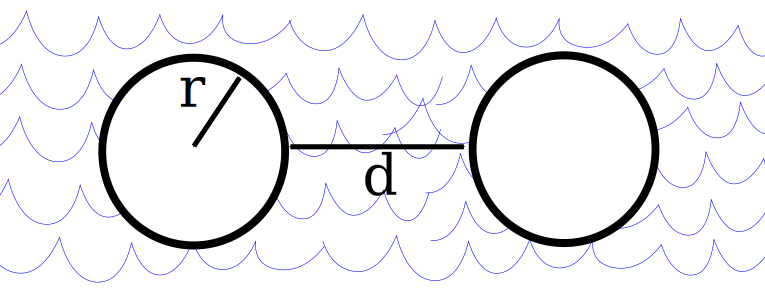
\includegraphics[width=\columnwidth]{figs/rods-diagram}
\end{center}
\caption{ Cross section schematic for two hydrophobic rods immersed in water.
The radius and separation are shown.}
\label{fig:rods}
\end{figure}

\begin{figure}
\begin{center}
\includegraphics[width=\columnwidth]{figs/density-rods-in-water}
\end{center}
\caption{ Density profiles illustrating the transition from vapor 
to liquid water between the rods. The radius is 0.5~nm, the top figure is at a separation of 0.2~nm and the
bottom is 0.4~nm. Figures~\ref{fig:rods-energy-vs-distance}~and~\ref{fig:energy-rods} show
the energy for these and other separations.}
\label{fig:density-rods}
\end{figure}

\begin{figure}
\begin{center}
\includegraphics[width=\columnwidth]{figs/energy-rods}
\end{center}
\caption{ Free energy, internal energy, and the entropic energy contribution versus
separation for two hydrophobic rods of radii 0.5~nm. All energies are arbitrarily
set to go to zero at large separations. }
\label{fig:energy-rods}
\end{figure}

\begin{figure}
\begin{center}
\includegraphics[width=\columnwidth]{figs/rods-energy-vs-distance}
\end{center}
\caption{ Energy versus separation for two hydrophobic rods ranging in radius from
0.3~nm to 0.9~nm. All were arbitrarily set to go to zero at large separations. The
transition corresponds to the phase change from
vapor to liquid between the rods as pictured in the density profiles in 
Figure~\ref{fig:density-rods}. }
\label{fig:rods-energy-vs-distance}
\end{figure}

We now look at the more interesting problem of two rods in water. We continue to
use hydrophobic rods of various radii at separation $d$ (see Figure~\ref{fig:rods}), ranging from $d=0$ 
(touching rods) to about 1~nm. At small
separations ($d<2$~-~4~nm) there is only vapor between the rods. As the rods are
pulled apart, the vapor region expands until some critical separation is
reached and liquid water fills the region between the rods. Figure~\ref{fig:density-rods} 
shows density profiles before and after this transition
for rods of radius 0.5~nm. This critical separation for the transition to liquid depends
somewhat on the radii of the rods, and is about 0.25~nm for the rods in Figure~\ref{fig:density-rods}.
Since we are looking at only hard-walled
non-interacting rods, the critical separation for this transition will be
different than any system where there is an appreciable force between rods. 
The density oscillations  around the rods are very similar to
those for the single hydrophobic rod in water, as seen in Figure~\ref{fig:density-single-rod}.
The oscillations around the two rods at small separation looks as if the two rods were one
solid object shaped \fixme{racetrack shaped?}.

For one set of rods (radii of 0.5~nm) the free energy is plotted with the internal energy
and the entropic energy contribution, where all are in units of energy per length 
(see Figure~\ref{fig:energy-rods}). The free energy slightly increases as the separation
goes from 0 to the critical separation (0.25~nm) and then is approximately constant at
larger separations. Since there is no repulsive interaction between the rods, there is no
large energy increase when the rods touch. The entropy has a minimum just before the rods
transition to let liquid between them. As the rods separate starting from zero, the area 
between them containing vapor increases and there is less overall volume for the 
surrounding liquid water to occupy and thus the entropy decreases. 
\needsworknow{More discussion of Figure~\ref{fig:energy-rods}, internal energy, how they add
together, etc.}

The free energy per length is compared for rods of several different radii
in Figure~\ref{fig:rods-energy-vs-distance}. For comparison, we arbitrarily adjust each data set such that the
free energy per length goes to zero at large separations. At large separations, the rods will 
simply act like two separate single rods in water and the total energy will
reach an asymptote proportional to the surface tension (similar to that shown in 
Figure~\ref{fig:energy-vs-diameter}).
The change in free energy per length at the point of transition increases as the radii of
the rods increases. The smallest radius we show is 0.3~nm, which shows only a slight increase in
free energy at the critical separation, while the largest radius has a more significant jump in free energy. 
We see that all the rods studied have the same behavior, with a positive linear relation between free energy
per length and the separation during the initial state where the rods have vapor between them. 
The slope of this line is equal to the force per length on the rods, which we calculate to be 144~mN/m, 
or twice the surface tension
found by the functional (see Figure~\ref{fig:surface-tension}).

Walther \emph{et al.}\cite{walther2004hydrodynamic} study the interactions between two
carbon nanotubes, which are very geometrically similar to our hydrophobic rods. 
They use molecular dynamics with Lennard-Jones potentials for
nanotubes of diameter 1.25~nm and separations ranging from about 0.3~nm to 1.5~nm.
They also find a drying transition occurs, and find it to be at separations near
0.9~-~1.0~nm\cite{walther2004hydrodynamic}. This is several times larger than
what we find for hydrophobic rods, as expected due to the carbon-carbon
interations between two nanotubes. 

%%%%%%%%%%%%%%%%%%%%%%%%%%%%%%%%%%%%%%%%%%%%%%%%%%%%%%%%%%%%
\section{Conclusion}

\needsworknow{Conclusions about slit, single rod, two hydrophobic rods (mostly). future uses}

\bibliographystyle{unsrt}
\bibliography{paper}% Produces the bibliography via BibTeX.

\end{document}

